\documentclass[a4paper, margin=1in]{article}
%\usepackage{CJK}
\usepackage{latexsym}
\usepackage{color}
\usepackage[x11names]{xcolor} % for a set of predefined color names, like LemonChiffon1
\usepackage{graphicx, float}\usepackage{graphicx}
\usepackage{algorithmic}
\usepackage{algorithm}
%\usepackage{algpseudocode}
%\usepackage[colorlinks]{hyperref}
\usepackage[toc,page]{appendix}
\usepackage{bm}
\setlength{\oddsidemargin}{-0.0in}
\setlength{\evensidemargin}{-0.0in} \setlength{\textwidth}{6.0in}
\setlength{\textheight}{9.0in} \setlength{\topmargin}{-0.2in}
%\usepackage[boxruled]{algorithm2e}

%\setlength{\leftmargin}{0.7in}
\usepackage{amssymb, graphicx, amsmath}  %  fancyheadings,
\usepackage{setspace}
\newcommand\qed{\qquad $\square$}
\newcommand{\nn}{\nonumber}

\usepackage{lipsum}

\usepackage{listings}
\lstset{
  basicstyle=\ttfamily,
  columns=fullflexible,
  frameround=fttt,
  breaklines=true,
  %postbreak=\mbox{\textcolor{red}{$\hookrightarrow$}\space},
}

\definecolor{mGreen}{rgb}{0,0.6,0}
\definecolor{mGray}{rgb}{0.5,0.5,0.5}
\definecolor{mPurple}{rgb}{0.58,0,0.82}
\definecolor{backgroundColour}{rgb}{0.95,0.95,0.92}

\lstdefinestyle{CStyle}{
basicstyle=\ttfamily,
language=C,
numberstyle=\tiny\color{mGray},
numbers=left,
frame=lines,
framexleftmargin=0.5em,
framexrightmargin=0.5em,
backgroundcolor=\color{LemonChiffon1},
showstringspaces=false,
escapeinside={(*@}{@*)},
}

\def \[{\begin{equation}}
\def \]{\end{equation}}
\def\proof{{\bf Proof:\quad}}
\def \endzm {\quad $\Box$}
\def\dist{\hbox{dist}}

\usepackage{tabularx,booktabs}
\newcolumntype{C}{>{\centering\arraybackslash\hsize=.5\hsize}X} % centered version of "X" type
\setlength{\extrarowheight}{1pt}
\usepackage{caption}% <-- added


\newcommand{\R}{\mathbb{R}}
%\newtheorem{yinli}{����}[section]
\newcommand{\D}{\displaystyle}
\newcommand{\T}{\textstyle}
\newcommand{\SC}{\scriptstyle}
\newcommand{\FT}{\footnotesize}

\usepackage{hyperref}
\newcommand\fnurl[2]{%
  \href{#2}{#1}\footnote{\url{#2}}%
}


%\newtheorem{theorem}{Theorem}[section]
%\renewcommand{\thetheorem}{\arabic{section}.\arabic{theorem}}
\newtheorem{definition}{Definition}
\renewcommand{\thedefinition}{\arabic{section}.\arabic{definition}}
\newtheorem{lemma}{Lemma}[section]
\renewcommand{\thelemma}{\arabic{section}.\arabic{lemma}}
\newtheorem{remark}{Remark}
\renewcommand{\theremark}{\arabic{section}.\arabic{remark}}
\newtheorem{proposition}{Proposition}[section]
\renewcommand{\theproposition}{\arabic{section}.\arabic{proposition}}
\newtheorem{corollary}{Corollary }[section]
\renewcommand{\thecorollary}{\arabic{section}.\arabic{corollary}}
\renewcommand{\theequation}{\arabic{section}.\arabic{equation}}
\renewcommand{\baselinestretch}{1.35}
\newtheorem{exam}{Example}[section]
\renewcommand{\theexam}{\arabic{section}.\arabic{exam}}
\newtheorem{theo}{Theorem}[section]
\renewcommand{\thetheo}{\arabic{section}.\arabic{theo}}

% Define a \HEADER{Title} ... \ENDHEADER block
\makeatletter
\newcommand{\HEADER}[1]{\ALC@it\underline{\textsc{#1}}\begin{ALC@g}}
\newcommand{\ENDHEADER}{\end{ALC@g}}
\makeatother

\newcommand{\argmin}{\operatornamewithlimits{argmin}}
\newcommand{\argmax}{\operatornamewithlimits{argmax}}

\usepackage{url} % to make url in bibtex shows up

% Create a command to cleanly insert a snippet with the style above anywhere in the document
\newcommand{\insertcode}[2]{\begin{itemize}\item[]\lstinputlisting[caption=#2,label=#1,style=CStyle]{#1}\end{itemize}} % The first argument is the script location/filename and the second is a caption for the listing

\begin{document}
%\begin{CJK*}{GBK}{song}

\begin{center}

{\LARGE \bf CS380L: Advanced Operating Systems Lab \#1}\\

\vskip 25pt
 {Zeyuan Hu \footnote{30 hours spent on this lab.}, iamzeyuanhu@utexas.edu }\\
\vskip 5pt
{\small EID:zh4378 Spring 2019 }

\end{center}

\begin{spacing}{1.5}
\section{Environment} \label{environment}

Unless otherwise noted, we use a Linux server for all the experiments. The server has 4 Intel(R) Xeon(R) CPU E3-1220 v5 @ 3.00GHz processors and 16GB of memory, and runs Ubuntu 16.04.2 LTS (kernel version 4.11.0). The CPU has 32KB of L1 data cache per core (8-way set associative) (found through \lstinline!getconf -a | grep CACHE!). In addition, it has two-level TLBs. The first level (data TLB) has 64 entries (4-way set associative), and the second level has 1536 entries for both instructions and data (6-way set associative) (found through \lstinline!cpuid | grep -i tlb!).

\section{Memory map}

\lstinline|/proc/[pid]/maps| file contains process \lstinline|[pid]|'s mapped memory regions and their access permissions \cite{proc_man}. We use
the following code to read content of \lstinline|/proc/self/maps| file \footnote{see \texttt{memory\_map.c} for complete code}:

%\insertcode{"../src/memory_map.c"}{Code for memory map task}
\begin{lstlisting}[style=CStyle]
sprintf(filepath, "/proc/%u/maps", (unsigned)getpid());
FILE *f = fopen(filepath, "r");

printf("%-32s %-8s %-10s %-8s %-10s %s\n", "address", "perms", "offset", "dev", "inode", "pathname");
while (fgets(line, sizeof(line), f) != NULL) {
     sscanf(line, "%s%s%s%s%s%s", address, perms, offset, dev, inode, pathname);
     printf("%-32s %-8s %-10s %-8s %-10s %s\n", address, perms, offset, dev, inode, pathname);
}
fclose(f);
\end{lstlisting}

In the file, each line corresponds to a mapped memory region. There are six columns of each line, which represent six properties of the mapped memory region: \texttt{address}, \texttt{perms}, \texttt{offset}, \texttt{dev}, \texttt{inode}, and \texttt{pathname}. The result of running \texttt{memory\_map.c} is below:

\begin{figure}
	\centering
	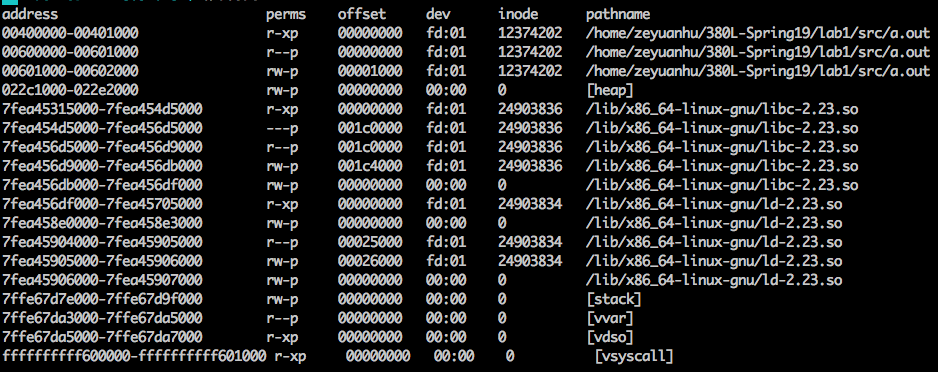
\includegraphics[scale=0.5]{memory_map.png} 
	\caption{Output of memory\_map.c}
	\label{memory_map}
\end{figure}

The \texttt{address} field gives range of virtual memory address of the mapped memory region. Access permission of each memory region is indicated by \texttt{perms} field. 
There are four bits in the field: \texttt{rwx} represents read, write, and executable respectively; the last bit (\texttt{p} or \texttt{s}) represents whether the region is private or shared. \texttt{offset} field represents the offset in the mapped file. \texttt{dev} field indicates the device (represented with format of \texttt{major:minor}) that the mapped file resides . There are two kinds of value in this column for our case: \texttt{fd:01} and \texttt{00:00}. The former one is the device id (in hex) of \texttt{/} (checked with \lstinline|mountpoint -d /|) and the latter one represents no device associated with the file.
\texttt{inode} field represents the inode number of the file on the device. \texttt{0} means no file is associated with the mapped memory region. \texttt{pathname} field gives the absolute path to the file associated with the mapped memory region. It can be some special values like \texttt{[heap]}, \texttt{[stack]}, \texttt{[vdso]}, etc.

To locate the start of the text section of the executable, we invoke \texttt{objdump -h} on the binary and get \texttt{0000000000400600}.  Output of \texttt{/proc/self/maps} shows that the start address of \texttt{libc} is \texttt{7fea45315000}. The reason for these two addresses are different is \texttt{libc} is dynamic loaded library, which is loaded during the runtime of executable, which is not compiled and linked as part of executable. The code segment contains the executable instruction, not the dynamic loaded library.

One interesting thing happens between runs of the executable: the content of \texttt{/proc/self/maps} is different. Addresses of all mapped memory regions are different except for the regions mapped to the executable and \texttt{[vsyscall]}. The root cause behind this phenomenon is Address Space Layout Randomization (ASLR) \cite{aslr} for programs in user space. This feature is enabled by default and can be seen via the content of \lstinline|/proc/sys/kernel/randomize_va_space| file. In our case, the value is 2, which means the positions of stack itself, virtual dynamic shared object (VDSO) page, shared memory regions, and data segments are randomized \cite{aslr2}.

\section{Getrusage}

To get resource usage of the current process, we use \texttt{getrusage} \cite{getrusage_man}. The result is stored in \texttt{rusage} struct. Not all fields of the struct
are completed: unmaintained fields are set to zero by the kernel. Those fields exist for compatibility with other systems purpose. The following code instantiates \texttt{rusage} struct and print all the maintained fields \footnote{complete code can be seen in \texttt{getrusage.c}}:

\begin{lstlisting}[style=CStyle]
struct rusage usage;
if (getrusage(RUSAGE_SELF, &usage) != 0) {
    perror("getrusage");
    return 0;
}

// user CPU time used
printf("utime = %ld.%06ld s\n", usage.ru_utime.tv_sec,
usage.ru_utime.tv_usec);
// system CPU time used
printf("stime = %ld.%06ld s\n", usage.ru_stime.tv_sec,
usage.ru_stime.tv_usec);
// maximum resident set size
printf("maxrss = %ld KB\n", usage.ru_maxrss);
// page reclaims (soft page faults)
printf("minflt = %ld\n", usage.ru_minflt);
// page faults (hard page faults)
printf("majflt = %ld\n", usage.ru_majflt);
// block input operations
printf("inblock = %ld\n", usage.ru_inblock);
// block output operations
printf("oublock = %ld\n", usage.ru_oublock);
// voluntary context switches
printf("nvcsw = %ld\n", usage.ru_nvcsw);
// involuntary context switches
printf("nivcsw = %ld\n", usage.ru_nivcsw);
\end{lstlisting}

man page of \texttt{getrusage} explains the meaning of each field \cite{getrusage_man} in details. \texttt{utime} and \texttt{stime} are about CPU time usage; \texttt{minflt} and \texttt{majflt} are related to page faults; \texttt{maxrss} represents the maximum size of working set; \texttt{inblock} and \texttt{oublock} are about file system I/O. 

\section{perf\_event\_open} 

We first check the support of \lstinline|perf_event_open| interface by checking the existence of \lstinline|/proc/sys/kernel/perf_event_paranoid|, which is true in our case (value is set to \texttt{2}). In Linux, \lstinline|perf_event_open| interface \cite{perf_event_open_man} is used to setup performance monitoring. Specifically, it provides an interface that allows user to access 
various events (i.e., events counted by performance counters \cite{hardware_counter}). \lstinline|perf list| gives available events on current machine. Counters related to cache in our machine is shown in Figure \ref{counters}. We are interested in counters related to L1 data cache and data TLB. As shown in Figure \ref{counters}, we have counters for number of times the L1 cache was accessed for data (\texttt{L1-dcache-loads}), the number of those access that resulted in a cache miss (\texttt{L1-dcache-load-misses}), and write access of L1 data cache (\texttt{L1-dcache-stores}). Similarly, for data TLB, we have read access (\lstinline|dTLB-loads|), read miss (\lstinline|dTLB-load-misses|), write access (\lstinline|dTLB-stores|), and write miss (\lstinline|dTLB-store-misses|).


\begin{figure}	
	\centering
	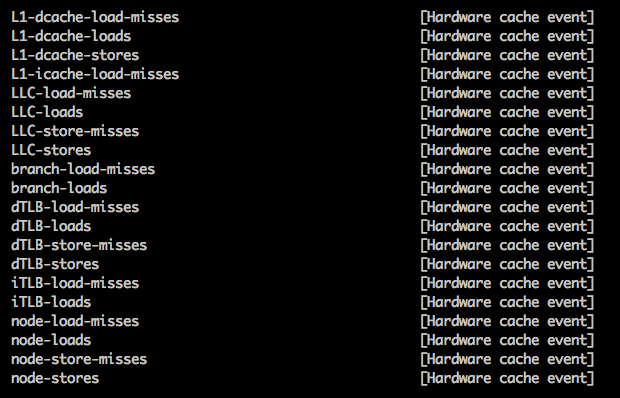
\includegraphics[scale=0.5]{counters.png} 
	\caption{Part of output of \texttt{perf list} related to cache}
	\label{counters}
\end{figure}

According to man page \cite{perf_event_open_man}, there is no glibc wrapper for 
\lstinline|perf_event_open| system call. However, we can wrap it on our own as the following:

\begin{lstlisting}[style=CStyle]
static long perf_event_open(struct perf_event_attr *hw_event, pid_t pid, int cpu, int group_fd, unsigned long flags) {
  return syscall(__NR_perf_event_open, hw_event, pid, cpu, group_fd, flags);
}
\end{lstlisting}

Using the \texttt{syscall} does not mean there is a syscall opcode in the program. Figure \ref{perf_event_open_dump} shows \texttt{perf\_event\_open} section of 
\texttt{objdump -d}. Using \texttt{syscall} function will have \texttt{perf\_event\_open} system call number compiled in the program. In this case, the system call number 
of \texttt{perf\_event\_open} is 298 (can be checked in \texttt{arch/x86/entry/syscalls/syscall\_64.tbl} of the Linux kernel source tree), which is \texttt{\$0x12a} in hex.

\begin{figure}	
	\centering
	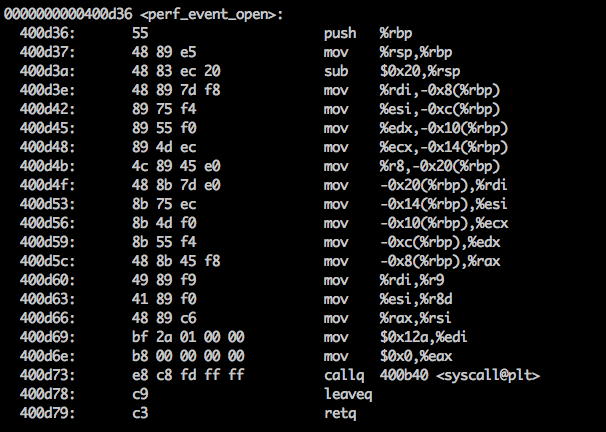
\includegraphics[scale=0.5]{perf_event_open_dump.png} 
	\caption{\texttt{perf\_event\_open} section of \texttt{objdump -d} output}
	\label{perf_event_open_dump}
\end{figure}

We want to monitor the following events: read, write, read miss for level 1 data cache and
read miss, write miss for data TLB. A call to \lstinline|perf_event_open| gives a file descriptor that corresponds to one event being measured.  We can use \texttt{ioctl} interface to control the counters and read file descriptors to obtain counter vales. The following code highlights the usage of \lstinline|perf_event_open| interface to measure
all five events for trivial \texttt{printf} \footnote{complete code can be seen in \texttt{perf\_event\_open\_usage.c}}.

\begin{lstlisting}[style=CStyle]
int hw_cache_perf_event_open(int group_fd, int cache_id, int cache_op_id,
int cache_op_result_id) {
  struct perf_event_attr pe;
  memset(&pe, 0, sizeof(struct perf_event_attr));
  pe.type = PERF_TYPE_HW_CACHE;
  pe.size = sizeof(struct perf_event_attr);
  pe.config = cache_id | (cache_op_id << 8) | (cache_op_result_id << 16);
  pe.disabled = 0;
  if (group_fd == -1) {
    pe.disabled = 1;
  }
  pe.exclude_kernel = 1;
  pe.exclude_hv = 1;
  int fd = perf_event_open(&pe, 0, cpu_id, group_fd, 0);
  if (fd == -1) {
    perror("perf_event_open");
    exit(EXIT_FAILURE);
  }
  return fd;
}

int main(int argc, char **argv) {

  int l1_read_access_fd = hw_cache_perf_event_open(
      -1, PERF_COUNT_HW_CACHE_L1D, PERF_COUNT_HW_CACHE_OP_READ,
      PERF_COUNT_HW_CACHE_RESULT_ACCESS);
  int leader_fd = l1_read_access_fd;

  int l1_read_miss_fd = hw_cache_perf_event_open(
      leader_fd, PERF_COUNT_HW_CACHE_L1D, PERF_COUNT_HW_CACHE_OP_READ,
      PERF_COUNT_HW_CACHE_RESULT_MISS);
  int l1_write_access_fd = hw_cache_perf_event_open(
      leader_fd, PERF_COUNT_HW_CACHE_L1D, PERF_COUNT_HW_CACHE_OP_WRITE,
      PERF_COUNT_HW_CACHE_RESULT_ACCESS);
  int tlb_read_miss_fd = hw_cache_perf_event_open(
      leader_fd, PERF_COUNT_HW_CACHE_DTLB, PERF_COUNT_HW_CACHE_OP_READ,
      PERF_COUNT_HW_CACHE_RESULT_MISS);
  int tlb_write_miss_fd = hw_cache_perf_event_open(
      leader_fd, PERF_COUNT_HW_CACHE_DTLB, PERF_COUNT_HW_CACHE_OP_WRITE,
      PERF_COUNT_HW_CACHE_RESULT_MISS);

  ioctl(leader_fd, PERF_EVENT_IOC_RESET, PERF_IOC_FLAG_GROUP);
  ioctl(leader_fd, PERF_EVENT_IOC_ENABLE, PERF_IOC_FLAG_GROUP);

  // Do the work that we want to analyze
  printf("Do some work that we want to measure here\n");

  ioctl(leader_fd, PERF_EVENT_IOC_DISABLE, PERF_IOC_FLAG_GROUP);

  uint64_t l1_read_miss = 0;
  uint64_t l1_read_access = 0;
  uint64_t l1_write_access = 0;
  uint64_t tlb_read_miss = 0;
  uint64_t tlb_write_miss = 0;

  read(l1_read_access_fd, &l1_read_access, sizeof(uint64_t));
  read(l1_read_miss_fd, &l1_read_miss, sizeof(uint64_t));
  read(l1_write_access_fd, &l1_write_access, sizeof(uint64_t));
  read(tlb_read_miss_fd, &tlb_read_miss, sizeof(uint64_t));
  read(tlb_write_miss_fd, &tlb_write_miss, sizeof(uint64_t));

  close(l1_read_access_fd);
  close(l1_read_miss_fd);
  close(l1_write_access_fd);
  close(tlb_read_miss_fd);
  close(tlb_write_miss_fd);

  printf("[Performance counters]\n");
  printf("Data L1 read access: %" PRIu64 "\n", l1_read_access);
  printf("Data L1 write access: %" PRIu64 "\n", l1_write_access);
  printf("Data L1 read miss: %" PRIu64 "\n", l1_read_miss);
  printf("Data L1 read miss rate: %.5f\n",
         (double)l1_read_miss / l1_read_access);
  printf("Data TLB read miss: %" PRIu64 "\n", tlb_read_miss);
  printf("Data TLB write miss: %" PRIu64 "\n", tlb_write_miss);

  fflush(stdout);

  return 0;
}
\end{lstlisting}

File descriptors returned from calling \lstinline|perf_event_open| can be 
grouped together so that we can measure corresponding events simultaneously. There are five events we want to measure and as shown in the code above, we group them together and measure them at the same time. However, measuring all five events at the same time may not possible for some machine as CPU only has limited amount of machine specific registers (MSRs) for low-level performance counting. In our environment, this number is 8 \footnote{check via \lstinline!cpuid|grep 'number of counters per logical processor'!}. For the following experiment, we also want to lock our 
process onto a single processor. To achieve it, we use the following code:

\begin{lstlisting}[style=CStyle]
cpu_set_t set;
CPU_ZERO(&set);
CPU_SET(cpu_id, &set);
if (sched_setaffinity(0, sizeof(cpu_set_t), &set) == -1) {
	perror("sched_setaffinity");
	exit(EXIT_FAILURE);
}
\end{lstlisting}

Here, all counters we setup are associated with CPU specified by \lstinline|cpu_id|. We use \lstinline|sched_setaffinity| system call to set the CPU affinity of current process and ensure that it runs on CPU of \texttt{cpu\_id} only.

\section{Measuring memory access behavior}

\texttt{mmap} system call maps files or devices into memory. The created mapping can be file-backed or anonymous. File-backed mapping maps an area of the process's virtual memory to files (i.e., an area of the process's virtual memory is mapped to file-backed memory); reading those areas of memory causes the file read. Anonymous mapping is the opposite of file-backed mapping (i.e., not backed by file; an area of the process's virtual memory is mapped to anonymous memory). In this section, we experiment with both types of mappings. Since file-backed mapping can be shared or private, we have three memory mappings setup in our experiment: anonymous, file-based (private) and file-based (share).
In this experiment, we use \lstinline|MAP_POPULATE| flag. \lstinline|MAP_POPULATE| populates page tables for a mapping. For file-backed mapping, this means read-ahead on file, which reduce blocking on page faults later. In addition, we use \texttt{memset} to initialize the mapped region and \texttt{msync} to flush the change made to the file-backed memory back to file system whenever possible. 

We study the following code, which is used to access the mapped region:

\begin{lstlisting}[style=CStyle]
#define CACHE_LINE_SIZE 64
int opt_random_access;  
void do_mem_access(char *p, int size) {
  int outer, locality, i;
  int ws_base = 0;
  int max_base = size / CACHE_LINE_SIZE - 512;
  for (outer = 0; outer < (1 << 20); outer++) {
    long r = simplerand() % max_base;
    if (opt_random_access) {
      ws_base = r;
    } else {
      ws_base += 512;
      if (ws_base >= max_base) {
        ws_base = 0;
      }
    }
    for (locality = 0; locality < 16; locality++) {
      volatile char *a;
      char c;
      for (i = 0; i < 512; i++) {
        a = p + ws_base + i * CACHE_LINE_SIZE;
        if (i % 8 == 0) {
          *a = 1;
        } else {
          c = *a;
        }
      }
    }
  }
}
\end{lstlisting}

\lstinline|simplerand()| is a function generates random number. A global variable \lstinline|opt_random_access| is used to specify the
memory access to be sequential or random. Specifically, \lstinline|db_mem_access()| routine will access a working set consists of
512 consecutive cache lines. Among those 512 cache lines, $\frac{1}{8}$ will be write access and $\frac{7}{8}$ will be read access. The
same working set is accessed 16 times. The whole routine will work on $2^{20}$ working sets. Working sets are selected either sequentially
or in random (specified by \lstinline|opt_random_access|). In sequential access case, offset between working sets is 512 (e.g., since there
are 512 cache lines of a set). In random access case, the start(i.e., base) of working set is selected randomly based on the number generated by \lstinline|simplerand()|. \lstinline|simplerand()| is called no matter the sequential memory access or random access because we want to keep the
experiment results difference only due to the memory access pattern difference. In other words, we want to have both memory access patterns have the same function call and context switch overheads (caused by calling \lstinline|simplerand()|).

We study \lstinline|db_mem_access()| behavior on a VM with 2GB of memory and 4 virtual CPU cores. The VM runs Ubuntu 18.10 with kernel version 4.19.6. \lstinline|-cpu host| is added as part of QEMU option to ensure our VM can access performance counters. We allocate 1GB buffer via \texttt{mmap} as input for \lstinline|do_mem_access|.  To ensure 
the repeatable result, we flush the level 1 data cache by accessing a 16MB buffer before calling \lstinline|do_mem_access|. We invoke \texttt{getrusage}  just before and after \lstinline|do_mem_access| to collect resource usage statistics of initialization code and \lstinline|do_mem_access|. We run the program 5 times and calculate mean and stand deviation of statistics \footnote{We compile our program with \texttt{-O2} to prevent any unwanted memory access from the generated executable}. We also submit the raw results along with this report.

\begin{figure}	
	\centering
	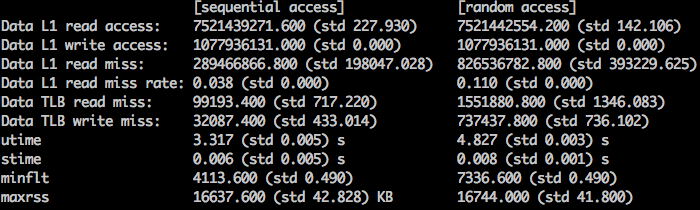
\includegraphics[scale=0.65]{sequential_random_anonymous} 
	\caption{The statistics of sequential and random memory accesses with anonymous mapped memory regions}
	\label{sequential_random_anonymous}
\end{figure}

We first compare sequential access and random access (indicated by \lstinline|opt_random_access|). We use anonymous mapped memory regions. Figure \ref{sequential_random_anonymous} shows  statistics for both cases \footnote{\texttt{majflt}, \texttt{inblock}, \texttt{oublock} are omitted because they are all 0}.  As shown in the figure, the ratio between read and write access is 7:1 for data L1 cache for both cases, which is as expected. The read miss rate in random access case is 3x higher than sequential access. For data TLB, read miss and write miss of random access is 15.6X and 23x higher than sequential access respectively. Random access runs 1.46x slower than sequential access. From those statistics, we can see that there is no significant difference in terms of runtime and miss rate of data L1 cache between random access and sequential access (e.g., miss rate for random access is around 0.1). In the case of sequential access, the number of data TLB read miss is about 99193, which is
396MB for 4KB page size. 396MB is smaller than the size of our buffer. If we take a look at the code, we notice \lstinline|max_base| in \lstinline|do_mem_access| restricts the maximum base address of the working set. If we take a look at how \lstinline|max_base| is initialized and the line we initialize \texttt{a}, we can see that the working set is essentially the first $\frac{1}{64}$ of the given buffer, which is 16MB, which matches with the value of \texttt{maxrss} we observed and is much lower than 1GB. Realizing this fact also explains why TLB miss count is lower than the total number of data pages \footnote{If we want to access all the allocated buffer (1GB), we should replace line 21 (\texttt{a} initialization) with \lstinline|a = p + (ws_base + i) * CACHE_LINE_SIZE;| }.

\begin{figure}	
	\centering
	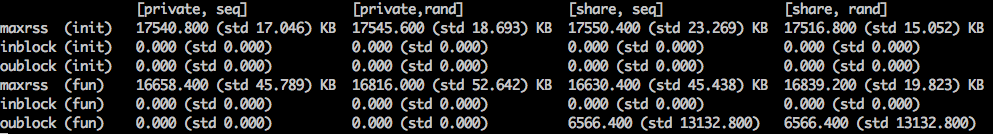
\includegraphics[scale=0.5]{share_private} 
	\caption{The statistics of sequential and random memory accesses with file-backed mapping with \lstinline|MAP_PRIVATE| and \lstinline|MAP_SHARED|. \texttt{fun} is a shorthand for \lstinline|do_mem_access|.}
	\label{share_private}
\end{figure}

In the next step, we experiment with file-based memory mappings.  In this part,
we only concern \texttt{maxrss}, \texttt{inblock}, and \texttt{oublock} because
the statistics related to data L1 cache and data TLB are generated with the same setup as anonymous mappings. In addition, statistics related to memory cache is not affected by the file-backed mapping. The statistics we have is shown in Figure \ref{share_private}. Compare to previous result, we notice there are 
large amount of \texttt{oublock} during \lstinline|do_mem_access| for file-backed mapping with \lstinline|MAP_SHARED|. This is intuitive as the changes to the file
have to be saved in shared mode. We notice that there is \texttt{inblock} is zero, 
which is due to the internal cache in Linux kernel for reading file.  \texttt{oublock} for both random access and sequential access under shared mode are exactly the same.  This may due to the fact that access pattern is not
significant for the shared mode as synchronization for internal file cache is needed no matter what memory access pattern we may encounter.

\begin{figure}	
	\centering
	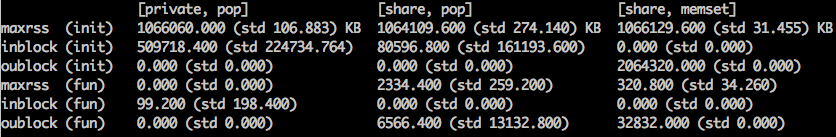
\includegraphics[scale=0.5]{populate_memset} 
	\caption{The statistics of file-backed mapping for \lstinline|MAP_POPULATE| and memset after buffer allocation. \texttt{fun} is a shorthand for \lstinline|do_mem_access|.}
	\label{populate_memset}
\end{figure}

In this experiment, we further examine \lstinline{MAP_POPULATE} flag and \texttt{memset} the mapped memory for initialization. Figure \ref{populate_memset} shows the statistics. Note that all the columns are from
the sequential memory access. With \lstinline|MAP_POPULATE| flag, the mapped memory will be populate page tables at the very beginning and perform read-ahead on the file. Thus we see the \texttt{maxrss} will match the allocated buffer size, which is around 1GB during the initialization. If the mapped memory 
is initialized with \texttt{memset} and then perform synchronization to the file system via \texttt{msync}, then there will be large amount of \texttt{oublock} during the initialization.

We also using \texttt{strace} to trace our program \footnote{we trace our program as \lstinline|strace ./memory_access 0 0 0 0 0 0|, where \lstinline|memory_access| is the executable from \lstinline|memory_access.c|}.  We find a system call \lstinline|arch_prctl(ARCH_SET_FS, 0x7f83a006d540) | in the printout. The system call means setting FS register to \texttt{0x7f83a006d540} \cite{arch_prctl_man}. FS register is a segment register with no specific processor-defined purpose and is given purpose by the OS. In Linux, FS register is for thread local storage. We can also see the system call \lstinline|access("/etc/ld.so.preload", R_OK)|, which tries to access \lstinline|/etc/ld.so.preload| file. This file contains ELF shared
objects, which are loaded before the execution of the program \cite{ld.so_man}. From the printout, we can see that this file is accessed before \texttt{libc.so} is loaded.

\section{Measuring memory access behavior with background activity}

In this section, we study the memory access behavior when there is a background activity. We use another process to allocate and access a large amount of memory to simulate background activity.

\begin{lstlisting}}[style=CStyle]
    int background_activity(void *unused) {
      long mem_size = get_mem_size();
      int page_sz = sysconf(_SC_PAGE_SIZE);
      printf(``Total memsize is %3.2f GBs\n'',
      (double)mem_size / (1024 * 1024 * 1024));
      fflush(stdout);
      char *p = mmap(NULL, mem_size, PROT_READ | PROT_WRITE,
      MAP_NORESERVE | MAP_PRIVATE | MAP_ANONYMOUS, -1, 0);
      if (p == MAP_FAILED) {
        perror(``Failed anon MMAP competition'');
        fflush(stdout);
        exit(EXIT_FAILURE);
      }

      int i = 0;
      while (1) {
        volatile char *a;
        long r = simplerand() % (mem_size / page_sz);
        char c;
        if (i >= mem_size / page_sz) {
          i = 0;
        }
        a = p + r * page_sz;
        c += *a;
        if (i % 8 == 0) {
          *a = 1;
        }
        i++;
      }
      return 0;
    }
\end{lstlisting}

\end{spacing}
\bibliographystyle{ieeetr}
\bibliography{report}
\end{document}

